% cap4.tex

\chapter{Análisis}
\label{c4}

Este capítulo inicia el análisis empírico del trabajo. Dado que la validación
que se persigue consiste en trasladar a un caso real un método que ya fue
aplicado a datos reales por sus propios autores, el análisis comienza por
reconstruir con precisión ese ejercicio de referencia, que es la aplicación de
\citeA{jalan_incentive-aware_2024} a la red de comercio internacional de la
OCDE. Sobre esa base se documenta después el levantamiento de datos realizado
para el programa Crédito Corfo Mipyme y se contrastan ambos casos, de modo que
la distancia entre uno y otro quede medida y no simplemente afirmada. El
capítulo cierra delimitando qué parte del análisis ya es concluyente con la
información disponible y qué parte queda condicionada a la entrega de datos
solicitada a CORFO.

\section{El ejercicio empírico de referencia. El caso de la OCDE}
\label{c4:ocde}

\subsection{Qué pregunta responde el ejercicio}
\label{c4:ocde-pregunta}

La aplicación empírica del modelo invierte la relación habitual entre datos y
teoría. Los datos no entran para alimentar un modelo que luego produce una red,
sino que la red observada es el dato de entrada y lo que se infiere son las
creencias de riesgo de los agentes, resumidas en la matriz de covarianzas
$\Sigma$. Esa inversión es la razón de ser del ejercicio, ya que $\Sigma$ no es
observable en ninguna fuente, mientras que la red de contratos sí lo es cuando
existe un registro de transacciones bilaterales.

El alcance de lo que puede inferirse está acotado de antemano. Según el
resultado de no identificabilidad recogido en la Sección~\ref{c24:identificacion},
una red $W$ dada no permite separar la terna de creencias $(M,\Gamma,\Sigma)$,
porque para cualquier par admisible de $\Gamma$ y $\Sigma$ existe un $M$ que
reproduce exactamente la misma red, y esa ambigüedad persiste aunque se observen
muchas redes generadas con los mismos $\Sigma$ y $\Gamma$. Por lo tanto el
ejercicio no pretende recuperar las creencias completas, sino únicamente
$\Sigma$ normalizada, bajo los supuestos de homogeneidad que se detallan más
adelante.

Esto explica por qué el conjunto de datos escogido es una red de comercio
internacional y no, por ejemplo, una cartera de créditos. El método exige una
magnitud bilateral que pueda leerse como el tamaño de un contrato entre dos
partes, medida repetidamente en el tiempo sobre el mismo conjunto de agentes y
disponible para prácticamente todos los pares posibles. El comercio bilateral
cumple las tres condiciones de manera natural.

\subsection{Los datos, su origen y su volumen}
\label{c4:ocde-datos}

Los datos provienen de las estadísticas de comercio internacional que publica la
OCDE en su portal estadístico, y cubren el comercio bilateral entre 46 economías
grandes, entre las que se incluyen las quince mayores del mundo por producto
interno bruto. La medición es trimestral y abarca desde el primer trimestre de
2010 hasta el segundo trimestre de 2022, lo que equivale a 50 trimestres.

La construcción del peso de cada arista merece atención porque es una decisión
metodológica y no un detalle de formato. El peso del par $\{i,j\}$ se define como
la suma de los flujos de $i$ hacia $j$ y de $j$ hacia $i$, de modo que la matriz
$W$ resulta simétrica y hay una sola cifra por par, tal como exige el punto
estable del modelo, en el que ambas partes acuerdan la misma cantidad. Dado que
no existe registro de comercio de un país consigo mismo, la red no tiene lazos
propios, y esa ausencia no se trata como dato faltante sino como arista
prohibida, mediante la extensión de la Proposición~1 al caso de aristas
prohibidas.

El volumen resultante se puede precisar. Con 46 agentes hay 1.035 pares
posibles, y con 50 trimestres se obtienen 49 matrices de diferencias
$\Delta W(t)$, de manera que el estimador dispone de 50.715 observaciones de par
por período frente a los 1.081 parámetros libres de $\Sigma$, es decir cerca de
47 ecuaciones por parámetro. La revisión directa del repositorio oficial del
artículo confirma las propiedades estructurales que el modelo supone, ya que las
49 matrices son exactamente simétricas y de diagonal nula, el 98,50~\% de las
entradas fuera de la diagonal es distinto de cero, 959 de los 1.035 pares son no
nulos en los 49 períodos y un solo par permanece en cero durante todo el
horizonte. La red es, en la práctica, completa.

Conviene registrar también cómo se recolectaron esos datos, porque es el punto
en que el caso de referencia y el caso chileno se separan desde el principio. La
recolección consistió en una única descarga desde un repositorio estadístico
internacional que ya publica la información organizada como panel, con
periodicidad uniforme, cobertura homogénea y una sola unidad de medida.

\subsection{El procedimiento aplicado a esos datos}
\label{c4:ocde-procedimiento}

El procedimiento, tal como está implementado en el repositorio oficial, se
compone de cinco pasos encadenados.

\begin{enumerate}
    \item Construcción de la secuencia de redes $W(t)$ y de sus diferencias
    $\Delta W(t)$ entre trimestres consecutivos.
    \item Proyección de cada diferencia con las matrices $\Psi_i$ de la
    topología, operación que anula las entradas correspondientes a aristas
    prohibidas y que en este caso solo afecta a la diagonal.
    \item Resolución del programa semidefinido de la Proposición~1, recogido en
    la Ecuación~\eqref{eq:prop1}, sobre las 49 diferencias, usando el solver SCS
    con cincuenta mil iteraciones, lo que según los propios autores toma del
    orden de treinta minutos.
    \item Regularización de la solución sumando $5\times 10^{-4}$ a la diagonal,
    paso necesario porque el uso posterior de $\hat\Sigma$ requiere invertir una
    matriz que el programa semidefinido tiende a devolver casi singular.
    \item Uso de $\hat\Sigma$ en dos análisis, que son el estudio de su espectro
    y el problema de detección de la fuente de un shock, este último resuelto a
    partir de la inversa de $\Sigma\otimes I + I\otimes\Sigma$ y evaluado con 500
    réplicas para cada tamaño de muestra.
\end{enumerate}

Es importante notar qué uso no se le da a $\hat\Sigma$ en el artículo. En
ninguno de los dos análisis se la emplea como estimación puntual de la matriz de
covarianzas verdadera, sino como insumo para una propiedad espectral y para una
tasa de acierto relativa. Esa distinción es relevante para el presente trabajo,
ya que la auditoría numérica del estimador realizada en este trabajo muestra que
el programa semidefinido publicado está sesgado cuando se lo evalúa como
estimación puntual, con un error relativo que se estanca en torno a 0,41 por
mucho que crezca el número de períodos, mientras que el estimador corregido con
el término jacobiano desciende hasta 0,10.
% TODO (autor) trasladar la auditoría completa del estimador al Anexo y citarla
% desde aquí con su \ref correspondiente.

\subsection{Los hallazgos del ejercicio}
\label{c4:ocde-hallazgos}

El primer hallazgo es que el espectro de la matriz inferida está fuertemente
sesgado. La reproducción realizada en este trabajo a partir de la matriz
publicada por los autores entrega un valor propio mayor de 0,2748 y uno menor de
$6,5\times 10^{-5}$, es decir una separación de 3,6 órdenes de magnitud, con los
cinco primeros valores propios concentrando el 73,5~\% de la traza y los diez
primeros el 90,7~\%, lo que equivale a un rango efectivo de 7,3. Dicho de otro
modo, las creencias de riesgo de 46 economías se comportan como si estuvieran
gobernadas por del orden de siete factores. El sesgo se agrava cuando la matriz
se estima con pocas muestras, y en particular el valor propio más pequeño cae
muy por debajo del segundo más pequeño.

El segundo hallazgo es la consecuencia práctica de lo anterior. Si un agente
quiere identificar cuál fue el contrato que recibió un shock de creencias,
observando únicamente cómo se movió la red, su tasa de acierto depende
críticamente de cuántas muestras sustentan la estimación de $\hat\Sigma$. Con 46
muestras la tasa de acierto exacto es nula y la de acertar dentro de los diez
contratos más movidos es de 0,008, mientras que con 96 muestras suben a 0,824 y
0,974 respectivamente, con crecimiento monótono entre ambos extremos. La lectura
que hacen los autores es que el sesgo espectral, combinado con el ruido, provoca
que los efectos indirectos de un cambio de creencias superen a los efectos
directos sobre el propio contrato afectado, lo que vuelve difícil la
intervención dirigida sobre una red real.

Conviene agregar una lectura propia que el artículo no explicita. El barrido de
tamaños de muestra llega hasta 96, mientras que la cota del Teorema~5, recogida
en la Ecuación~\eqref{eq:teorema5}, exige $\lceil n\log n\rceil$ muestras, que
para $n=46$ equivale a 177. El hecho de que la curva de acierto exacto aún no
sature dentro del rango explorado es por lo tanto coherente con esa cota y no
una anomalía del experimento.

La Figura~\ref{fig:ocde-resultados} reproduce ambos hallazgos a partir de los
archivos del repositorio oficial.

\begin{figure}[H]
    \centering
    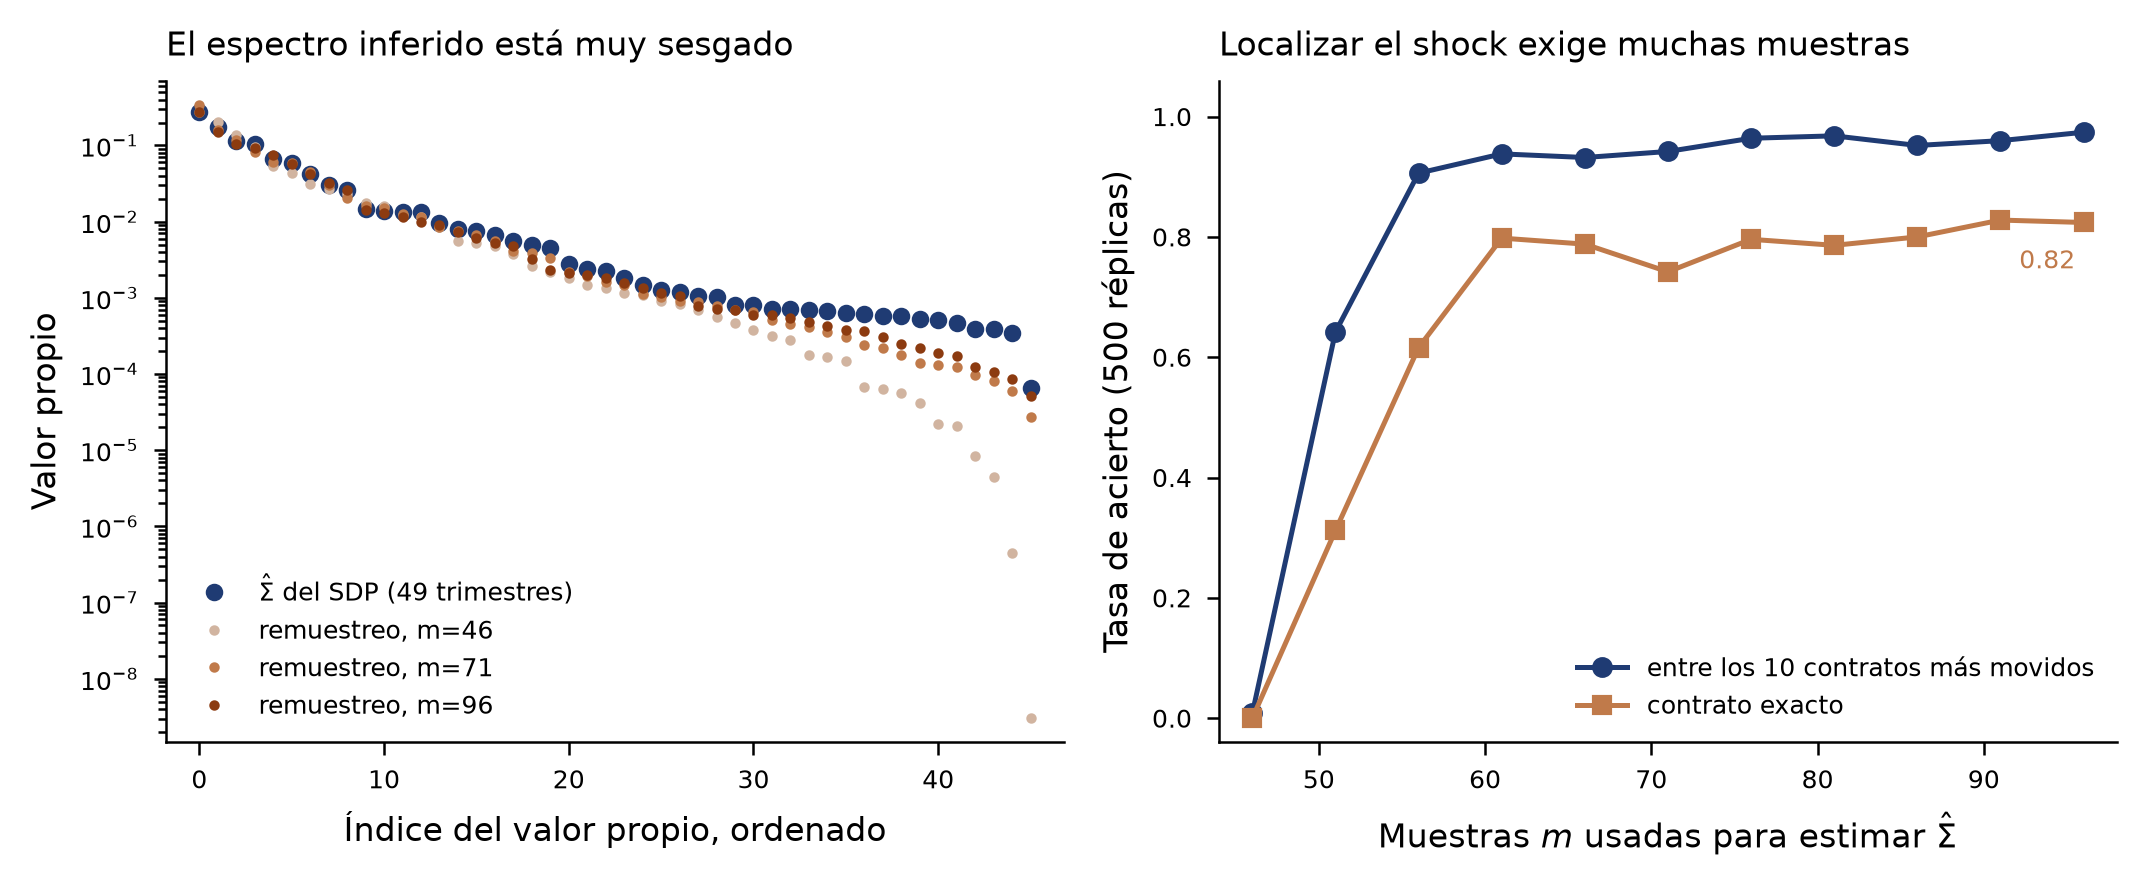
\includegraphics[width=\textwidth]{fig_jalan_ocde_resultados.png}
    \caption[Resultados del caso OCDE reproducidos]{Reproducción de los dos
    resultados empíricos del caso OCDE a partir del repositorio oficial de
    \citeA{jalan_incentive-aware_2024}. El panel izquierdo muestra el espectro de
    la matriz inferida por el programa semidefinido sobre 49 diferencias
    trimestrales, junto con el espectro de estimaciones construidas con $m$
    muestras. El panel derecho muestra la tasa de acierto en el problema de
    detección de la fuente, sobre 500 réplicas por tamaño de muestra.}
    \label{fig:ocde-resultados}
\end{figure}

\section{El levantamiento de datos del caso chileno}
\label{c4:levantamiento}

\subsection{Estrategia de búsqueda y fuentes recorridas}
\label{c4:levantamiento-fuentes}

La diferencia de partida con el caso de referencia es que no existe ningún
repositorio que publique la red del programa como panel. El panel debió
construirse documento a documento, y esa reconstrucción es en sí misma parte del
resultado de este trabajo, porque delimita lo que la información pública permite
afirmar. Se recorrieron cuatro familias de fuentes.

\begin{enumerate}
    \item Cuentas Públicas de CORFO entre 2014 y 2024, revisadas de forma
    íntegra. De ahí se obtuvo el desembolso de CORFO hacia los intermediarios en
    2019, 2020 y 2024, y la colocación de los intermediarios hacia las MiPyMEs en
    2016, 2019, 2020, 2021, 2023 y 2024. La cifra de 2017 corresponde a
    aprobación de líneas por parte del Comité Ejecutivo de Créditos y no a
    desembolso efectivo, el documento principal de 2018 es un escaneo sin capa de
    texto, y la Cuenta Pública de 2022 no reporta ninguna cifra monetaria del
    programa.
    \item Fichas de Monitoreo y Seguimiento de la Oferta Pública de DIPRES entre
    2019 y 2024, junto con el Informe de Detalle de Programas Sociales de cierre
    de 2021. Esta familia entrega la serie más completa del tramo entre CORFO y
    los intermediarios, cubriendo desde 2017 hasta 2024 y además desagregada por
    componente, es decir crédito, leasing y factoring.
    \item Portal estadístico de la Comisión para el Mercado Financiero. La
    revisión confirmó que la CMF no distingue el segmento MiPyME en sus series de
    tasas, ya que la única segmentación disponible es por tramo de monto en
    unidades de fomento, plazo y reajustabilidad. La serie más cercana a lo
    requerido es la estructura de colocaciones comerciales por evaluación de
    riesgo individual y grupal, disponible por banco desde febrero de 2019, que
    sin embargo es saldo de cartera y no flujo de desembolso.
    \item Portal de datos abiertos del Estado. La búsqueda programática con trece
    términos distintos no arrojó ningún conjunto de datos del programa, dado que
    la organización CORFO publica allí solo seis conjuntos, todos de 2012 y 2013 y
    referidos a instrumentos distintos.
\end{enumerate}

Una consecuencia metodológica de este levantamiento es que el estado de cada
celda pasa a ser parte del dato. Cada observación del panel se registra junto con
su fuente, su página y una marca que distingue lo observado de lo faltante, de
modo que el análisis posterior nunca trate como medición lo que en realidad es un
supuesto.

\subsection{El panel obtenido}
\label{c4:levantamiento-panel}

El panel resultante se muestra en la Figura~\ref{fig:panel-comparado}. Antes de
leerlo conviene fijar sobre qué conjunto de aristas se mide la cobertura, porque
no es único. El modelo dual tal como está especificado en la
Sección~\ref{c3:estructura} tiene tres aristas estructurales, que son CORFO con
el intermediario y el intermediario con la MiPyME en la red Tradicional, más el
banco comercial con la MiPyME en la red Alternativa, dado que CORFO y el
intermediario participan solo en la primera y el banco solo en la segunda. A
esas tres se agregan dos aristas que no forman parte de la especificación
original y que el diagnóstico de identificabilidad propone incorporar como
extensión de diseño, que son el fondeo bancario de los propios intermediarios y
las líneas que CORFO coloca a través de bancos comerciales. La grilla de la
figura se construye sobre ese conjunto extendido de cinco aristas, de modo que
las dos últimas filas no deben leerse como datos faltantes de la especificación
vigente sino como la información que haría falta si se adoptara la extensión.

Sobre esa grilla de nueve años hay nueve celdas observadas de cuarenta y cinco.
De las tres aristas estructurales, la que une al banco comercial con la MiPyME
está completamente vacía, mientras que las dos aristas de la red Tradicional
coinciden en 2019, 2020 y 2024, de los cuales solo 2019 y 2020 son años
consecutivos.

\begin{figure}[H]
    \centering
    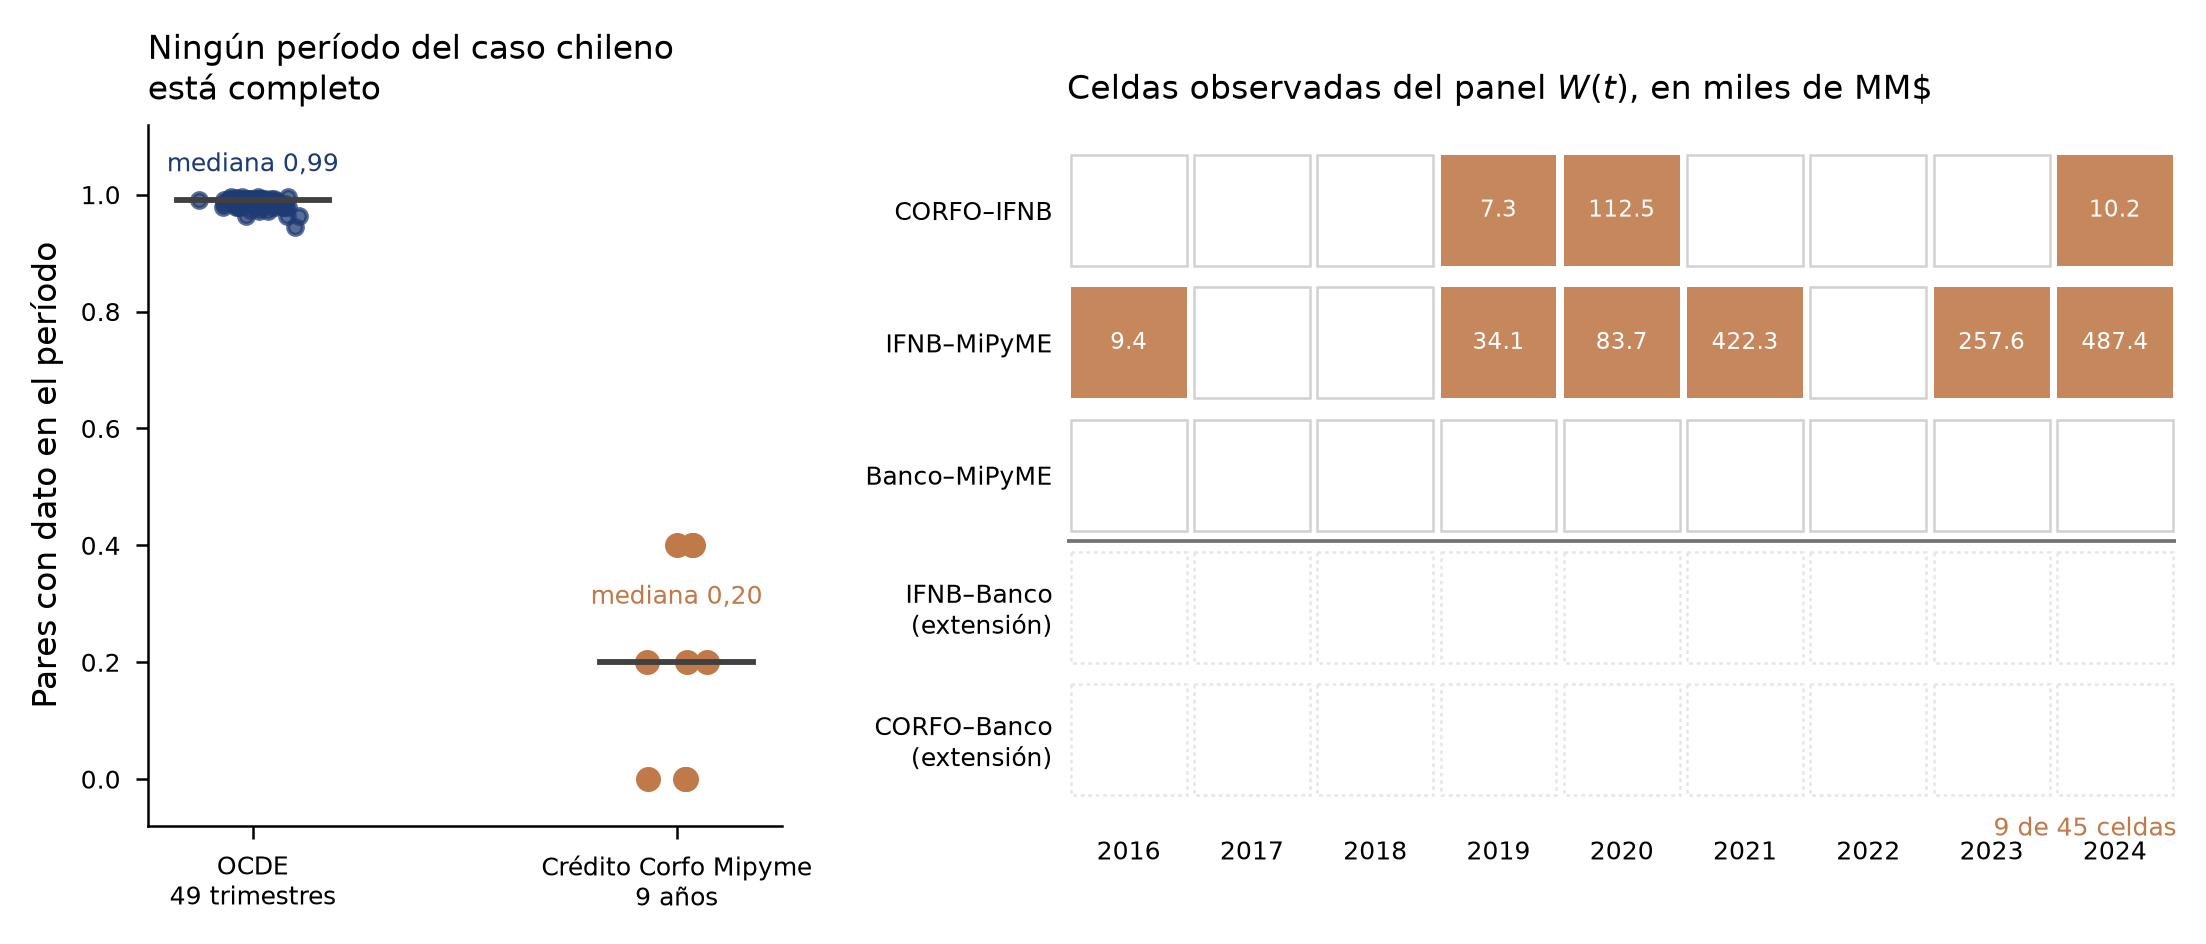
\includegraphics[width=\textwidth]{fig_panel_ocde_vs_corfo.png}
    \caption[Cobertura comparada de ambos paneles]{Cobertura del panel en ambos
    casos. El panel izquierdo compara, período a período, la fracción de pares
    con dato disponible. El panel derecho detalla la grilla del caso chileno, con
    las celdas observadas en miles de millones de pesos y las celdas faltantes en
    blanco. Las dos últimas filas de esa grilla corresponden a la extensión de
    diseño y no a aristas de la especificación vigente del modelo dual.}
    \label{fig:panel-comparado}
\end{figure}

El dato decisivo para el método no es sin embargo el número de celdas, sino el
número de diferencias utilizables, ya que el estimador de la Proposición~1 opera
sobre $W(t+1)-W(t)$ y una sola celda faltante elimina el período completo. Bajo
ese criterio el recuento depende de qué red se considere. Para la red de cuatro
agentes, en cualquiera de sus dos versiones, no hay ninguna diferencia
utilizable, porque ningún año tiene completas todas sus aristas. Restringiendo
la mirada a la red Tradicional por separado, que involucra únicamente a CORFO,
al intermediario y a la MiPyME, hay exactamente una diferencia utilizable, que
es la que va de 2019 a 2020, frente a los seis parámetros libres de la $\Sigma$
de tres agentes. Esa única diferencia tampoco alcanzaría aunque se dispusiera de
muchas más, ya que el rango de la información en esa cadena es de 3 sobre 6,
según se detalla en la Sección~\ref{c4:comparacion}.

\subsection{Obstáculos de comparabilidad detectados}
\label{c4:levantamiento-obstaculos}

Además de la cobertura, el levantamiento dejó al descubierto cuatro problemas que
afectan la comparabilidad de las cifras entre sí.

\begin{enumerate}
    \item Ambigüedad entre flujo y saldo. Las Cuentas Públicas reportan
    desembolsos, mientras que la serie bancaria más cercana de la CMF reporta
    saldos de cartera vigente, y el modelo trata la arista como una posición
    única, por lo que mezclar ambas naturalezas entre aristas rompe la
    comparabilidad.
    \item Multiplicidad de bases de pesos reales. Las fichas de DIPRES reexpresan
    cada año en la base del año de publicación, de modo que un mismo ejercicio
    aparece con cifras distintas según la ficha que se consulte. El gasto de 2018
    figura como 12.517,5 millones de pesos de 2020 y como 12.459,3 millones de
    pesos de 2021, mientras que el de 2019 figura como 7.519,0 y como 7.658,4 en
    esas mismas dos bases.
    \item Períodos parciales. La cifra de 2018 cubre entre enero y noviembre, y
    la de 2021 también, de manera que ninguna de las dos es comparable con un año
    completo sin un ajuste declarado.
    \item Distinción entre aprobación y desembolso. La única cifra disponible
    para 2017 corresponde a líneas de crédito aprobadas y no a montos girados.
\end{enumerate}

A estos cuatro se suma un problema de agregación. Las fuentes públicas reportan a
los intermediarios como un único agregado, de modo que la red observable tiene un
solo nodo intermediario, cuando en realidad el programa opera con varias
instituciones distinguibles entre sí.

\section{Comparación de los dos casos}
\label{c4:comparacion}

La Tabla~\ref{tab:comparacion-ocde-corfo} resume el contraste entre ambos
ejercicios en las dimensiones que el método vuelve relevantes.

\begin{table}[H]
    \centering
    \small
    \caption[Comparación entre el caso OCDE y el caso chileno]{Comparación entre
    el ejercicio empírico de \citeA{jalan_incentive-aware_2024} y el panel
    levantado para el programa Crédito Corfo Mipyme.}
    \label{tab:comparacion-ocde-corfo}
    \begin{tabular}{p{3.2cm}p{4.6cm}p{5.4cm}}
        \toprule
        Dimensión & Caso OCDE & Crédito Corfo Mipyme \\
        \midrule
        Agentes $n$ & 46 & 4 \\
        Pares posibles & 1.035 & 6 \\
        Aristas admisibles & 1.035, solo se prohíbe el lazo propio & 3 estructurales, más 2 en la extensión de diseño \\
        Períodos & 50 trimestres entre 2010 y 2022 & 9 años entre 2016 y 2024 \\
        Diferencias utilizables & 49 & 0 en la red de cuatro agentes y 1 en la red Tradicional sola \\
        Celdas observadas & 50.715 de 50.715 & 9 de 45 en la grilla extendida \\
        Entradas no nulas & 98,50 \% & no evaluable \\
        Parámetros de $\Sigma$ & 1.081 & 10 \\
        Ecuaciones por parámetro & 46,9 & 0 \\
        Rango de la información & 21 de 21 en el análogo completo con $n=6$ & 5 de 10 en la cadena de cuatro agentes y 3 de 6 en la red Tradicional sola \\
        Identificación de $\Sigma$ & sí & no \\
        Peso de la arista & suma de los flujos en ambos sentidos & desembolso en un solo sentido \\
        Medición & flujo comercial en una sola base & mezcla de flujo y saldo en cuatro bases distintas \\
        Obtención & descarga única desde un repositorio estadístico & reconstrucción documento a documento \\
        \bottomrule
    \end{tabular}
\end{table}

De esa comparación se desprenden tres diferencias, y conviene distinguirlas
porque no son todas igualmente reparables.

\paragraph{Diferencia de volumen.} Es la más visible y a la vez la menos grave,
ya que depende únicamente de la periodicidad y de la cobertura de la fuente. La
solicitud de información cursada a CORFO, que pide registros mensuales entre
enero de 2016 y diciembre de 2024, llevaría el panel de nueve observaciones
anuales a 108 períodos y 107 diferencias, con lo que el volumen dejaría de ser la
restricción activa.

\paragraph{Diferencia de topología.} Es la decisiva y no se repara con más datos
del mismo tipo. La red que entregan los registros de CORFO está formada por
CORFO, por los intermediarios y por las MiPyMEs, y es bipartita, puesto que
CORFO y las MiPyMEs quedan de un lado y los intermediarios del otro, sin ninguna
arista dentro de cada lado, mientras que la red de la OCDE es prácticamente
completa. En una red bipartita el residuo del estimador solo toca entradas de
$\Sigma$ dentro de cada lado, de modo que ninguna cantidad de meses ni de
intermediarios adicionales informa sobre el resto.

Esa misma lectura explica por qué la extensión de diseño descrita en la
Sección~\ref{c4:levantamiento-panel} sí repara la identificación, y conviene
distinguir el papel de cada una de sus dos aristas. El fondeo bancario de los
intermediarios une a dos agentes que están del mismo lado, de manera que es la
única de las dos que rompe la bipartición. Las líneas que CORFO coloca a través
de bancos comerciales, en cambio, cruzan de un lado al otro y por lo tanto no la
rompen, aunque el cálculo de rango muestra que de todos modos hacen falta,
puesto que solo con ambas aristas presentes a la vez el rango pasa de 18 a 21
sobre 21. El carácter bipartito de la red del programa es un aporte propio del
presente trabajo y no una consecuencia enunciada en la fuente, dado que los
resultados de identificación de dicho artículo se formulan para redes sin
aristas prohibidas.

\paragraph{Diferencia de homogeneidad de la medición.} El Supuesto~1 exige que la
volatilidad de las creencias sea la misma en todas las aristas. En la red de la
OCDE todas las aristas son comercio entre pares del mismo tipo, mientras que en
el programa el tramo que va de CORFO hacia los intermediarios es administrado,
porque las tasas las fija un comité y la asignación se hace por licitación, y por
lo tanto no es un proceso de creencias de mercado. Este es el supuesto más frágil
del traslado y debe declararse como tal.

\subsection{Una precisión sobre el uso del Teorema 5}
\label{c4:precision-teorema5}

El diagnóstico muestral del Capítulo~\ref{c3} aplica la cota del Teorema~5 al
largo del panel disponible. Corresponde precisar esa lectura, porque el teorema y
el panel se refieren a objetos distintos. La cantidad $m$ que aparece en la
Ecuación~\eqref{eq:teorema5} es el número de muestras de retornos con que cada
agente estima su propia covarianza $\hat\Sigma_i$, y el resultado acota cuánto se
degrada el factor de amortiguación seguro de las negociaciones bilaterales cuando
esa estimación es imperfecta. En cambio el largo del panel $W(t)$ es el insumo de
la ruta alternativa, que es la Proposición~1 de la Ecuación~\eqref{eq:prop1},
donde lo que se estima es una $\Sigma$ común a partir de los incrementos de la
red observada. La propia Sección~\ref{c24:identificacion} presenta ambas rutas
como alternativas entre sí.

La precisión tiene dos consecuencias. La primera es que la cota de seis
observaciones no es el criterio que decide si el panel alcanza, puesto que el
criterio pertinente es cuántas diferencias completas $\Delta W$ existen, y hoy
son cero. La segunda es que el Teorema~5 supone explícitamente que no hay aristas
prohibidas, condición que la red del programa no cumple, de modo que su cota no
es directamente aplicable al caso. El diagnóstico de insuficiencia del panel se
sostiene igualmente, pero su fundamento correcto es la combinación de ausencia de
diferencias utilizables y déficit de rango por bipartición, y no el
incumplimiento de la cota del Teorema~5.

\section{Alcance del análisis con la información disponible}
\label{c4:alcance}

El contraste anterior permite ordenar el trabajo restante en tres niveles, según
de quién dependa cada uno.

\paragraph{Resultados que ya son concluyentes.} No dependen de ninguna entrega
pendiente y corresponden al diagnóstico de identificabilidad, es decir la
bipartición de la red del programa y el déficit de rango que de ella se sigue, la
caracterización de qué entradas de $\Sigma$ serían recuperables y cuáles no, y la
auditoría del estimador publicado junto con la corrección propuesta.

\paragraph{Resultados que se desbloquean con la entrega de CORFO.} Con registros
mensuales e intermediarios distinguidos uno a uno, el panel pasa a 107
diferencias y la red a $1+k+1$ nodos, lo que permite estimar las covarianzas
entre pares de intermediarios y la covarianza entre CORFO y la MiPyME, que son
precisamente las entradas que el cálculo de rango señala como recuperables en una
red bipartita.

\paragraph{Resultados que requieren fuentes externas a CORFO.} La identificación
completa de $\Sigma$ exige dos aristas que deben levantarse simultáneamente, que
son el fondeo bancario de los propios intermediarios, única de las dos que rompe
la bipartición, y las líneas que CORFO coloca a través de bancos comerciales. La
primera no pertenece al ámbito de CORFO y debe buscarse en la información de la
CMF o en los estados financieros de los intermediarios.

Mientras esas entregas no se concreten, el análisis que este capítulo habilita es
de naturaleza comparativa y estructural, en el sentido de que establece qué exige
el método, cuánto de eso cubre la información pública chilena y qué faltaría
exactamente para cerrar la brecha, lo que constituye el punto de partida del
análisis cuantitativo que continúa en las secciones siguientes.
